\documentclass[11pt,a4paper]{article}
\usepackage[a4paper,margin=28mm,headheight=16pt]{geometry}
\usepackage[T1]{fontenc}
\usepackage{lmodern,microtype}
\usepackage{amsmath,amssymb,amsthm,mathtools}
\usepackage{booktabs,tabularx,array,multirow}
\usepackage{graphicx,xcolor,tikz}
\usepackage[font=small,labelfont=bf]{caption}
\usepackage{enumitem}
\usepackage{fancyhdr}
\usepackage[numbers,sort&compress]{natbib}
\usepackage[colorlinks=true,linkcolor=blue!45!black,citecolor=blue!45!black,urlcolor=blue!45!black]{hyperref}
\hypersetup{pdftitle={Prime-Gap Types and the Multitype Rescue Problem for Goldbach Representations},pdfauthor={Paul A. Bilokon}}
\setlength{\parskip}{4pt}
\setlength{\parindent}{12pt}
\setlist[itemize]{itemsep=2pt,topsep=3pt}
\pagestyle{fancy}
\fancyhf{}
\fancyhead[L]{\small Prime-gap types and Goldbach rescue}
\fancyhead[R]{\small Research note}
\fancyfoot[C]{\thepage}
\newtheorem{theorem}{Theorem}[section]
\newtheorem{proposition}[theorem]{Proposition}
\newtheorem{lemma}[theorem]{Lemma}
\newtheorem{corollary}[theorem]{Corollary}
\theoremstyle{definition}
\newtheorem{definition}[theorem]{Definition}
\newtheorem{conjecture}[theorem]{Conjecture}
\theoremstyle{remark}
\newtheorem{remark}[theorem]{Remark}
\newcommand{\PP}{\mathbb P}
\newcommand{\ind}{\mathbf 1}
\newcommand{\sg}{\mathfrak S}
\newcommand{\Z}{\mathbb Z}
\newcommand{\Ct}{\mathcal C}
\title{\bfseries Prime-Gap Types, Crossed Rescues, and the Limits of a Multitype Induction for Goldbach Representations\\[5pt]
\large Exact Transition Identities, Singular-Series Structure, and Computational Evidence}
\author{Paul A. Bilokon}
\date{Working manuscript --- 19 October 2026}
\begin{document}
\maketitle
\begin{abstract}
We investigate an inductive approach to binary Goldbach representations that augments existence with \emph{types} determined by prime-pair gaps.  A fixed pair of gaps $(6k+2,6k+4)$ provides an exact two-endpoint replacement between the consecutive even integers $6r+2$ and $6r+4$, and four associated primes produce a family of four additive targets.  We derive a mixed convolution for each rescue type, a sum-and-difference identity in signed imbalance coordinates, and an exact identity for the total number of oriented rescue configurations.  We establish local admissibility and a uniform finite-sieve lower bound simultaneously for linearly many types, as well as explicit cross-type modular exclusions.  For general even prime gaps $(a,b)$, we give an orientation-aware generating-function formalism and a uniformly positive Euler-product singular series.  Computations for thirteen gap types through $r=300{,}000$ and a fully enumerated example at the complete reset $277\to278$ illustrate redundancy among rescue mechanisms.  The multitype renewal implication needed for an induction is isolated as a separate open conjecture.  None of the results proves Goldbach or any prescribed-gap prime-pair conjecture.
\end{abstract}
\noindent\textbf{Keywords.} Goldbach conjecture; prime pairs; twin primes; cousin primes; sieve methods; singular series; additive convolution; induction; arithmetic dynamics.\\
\textbf{2020 MSC.} 11P32, 11N36, 11N05.

\section{Introduction and scope}
The binary Goldbach conjecture asserts that every even integer $N\ge4$ is a sum of two primes.  The classical heuristic of Hardy and Littlewood \citep{HardyLittlewood1923} predicts the density of representations but has not yielded a universal proof.  We study a more structured question: can a representation at one even target \emph{force} a representation at the next target because the prime endpoints belong to specified prime-pair classes?

The motivating example is the complete reset between $554=2\cdot277$ and $556=2\cdot278$:
\begin{equation}\label{eq:example-tile}
239+313=552,\quad241+313=554,\quad239+317=556,\quad241+317=558.
\end{equation}
Here $(239,241)$ is a twin-prime pair and $(313,317)$ a cousin-prime pair.  The transition from $554$ to $556$ replaces \emph{both} endpoints.  We generalize this replacement rule to a hierarchy of fixed-gap types.

We carefully separate three levels of assertion: identities following from the definitions; local congruence and finite-sieve theorems, which do not require simultaneous primality; and existence or asymptotic conjectures about four actual primes.  In particular, the observed persistence of a finite family of rescue types does not supply a valid inductive step without an additional uniform renewal theorem.  This distinction is consistent with the obstacles familiar from sieve theory \citep{HalberstamRichert1974,Maynard2015}.

\section{Goldbach rows, resets, and four-prime tiles}
For integer $m\ge3$, define the ordered endpoint set
\begin{equation}
 S(m)=\{p\in\PP:2m-p\in\PP\}.
\end{equation}
The set is reflection-invariant: $p\in S(m)$ if and only if $2m-p\in S(m)$. A \emph{complete reset} at $m\to m+1$ means
\begin{equation}\label{eq:reset}
 S(m)\cap S(m+1)=\varnothing,
\end{equation}
which does \emph{not} mean that either row is empty.

\begin{proposition}[Exact complete-reset criterion]\label{prop:reset}
For every integer $r\ge2$,
\begin{equation}
 S(3r+1)\cap S(3r+2)=\varnothing
 \quad\Longleftrightarrow\quad 6r-1\notin\PP.
\end{equation}
\end{proposition}
\begin{proof}
A common endpoint $p$ gives primes $q=6r+2-p$ and $q+2=6r+4-p$. If $q>3$, the lower member $q$ of a twin pair satisfies $q\equiv-1\pmod6$, apart from no other exception, and hence $p\equiv3\pmod6$, forcing $p=3$. This gives $q=6r-1\in\PP$.  If $q=3$, then $p=6r-1\in\PP$. Conversely, if $6r-1$ is prime, then $p=6r-1$ belongs to both rows via complements $3$ and $5$.
\end{proof}

\begin{definition}[Oriented four-prime tile]
For $k\ge0$ and $i,j\ge1$, a \emph{type-$k$ tile} consists of the four primes
\begin{equation}\label{eq:tile-primes}
 u=6i-1,\quad u'=6(i+k)+1,\quad
 v=6j+1,\quad v'=6(j+k)+5.
\end{equation}
The first gap is $u'-u=6k+2$ and the second is $v'-v=6k+4$.
\end{definition}
Writing $r=i+j+k$, the four sums satisfy
\begin{equation}\label{eq:tile-targets}
 \begin{aligned}
 u+v&=6(r-k), &u'+v&=6r+2,\\
 u+v'&=6r+4, &u'+v'&=6(r+k+1).
 \end{aligned}
\end{equation}
Therefore $u'+v\mapsto u+v'$ is a forced two-endpoint rescue, increasing the target by precisely $2$.  For $k=0$, the four targets are four successive even integers.  For $k>0$ they are not four consecutive even integers; the middle two remain consecutive.

\begin{figure}[ht]
\centering
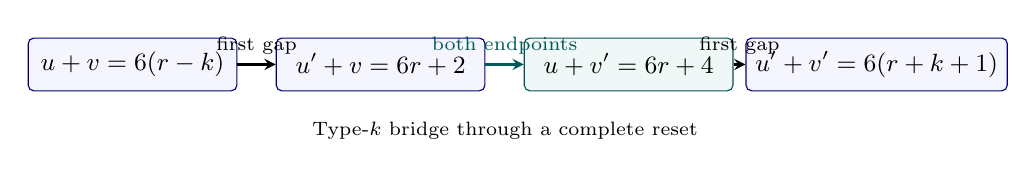
\begin{tikzpicture}[x=1cm,y=1cm,>=stealth]
\tikzset{box/.style={draw=blue!45!black,fill=blue!4,rounded corners=2pt,minimum width=2.65cm,minimum height=.67cm,align=center,font=\small}}
\node[box] (ll) at (0,0) {$u+v=6(r-k)$};
\node[box] (ul) at (3.15,0) {$u'+v=6r+2$};
\node[box,draw=teal!65!black,fill=teal!6] (lu) at (6.30,0) {$u+v'=6r+4$};
\node[box] (uu) at (9.45,0) {$u'+v'=6(r+k+1)$};
\draw[->,thick] (ll) -- node[above,font=\scriptsize] {first gap} (ul);
\draw[->,thick,teal!70!black] (ul) -- node[above,font=\scriptsize] {both endpoints} (lu);
\draw[->,thick] (lu) -- node[above,font=\scriptsize] {first gap} (uu);
\node[font=\scriptsize,below=7pt] at (4.73,-.36) {Type-$k$ bridge through a complete reset};
\end{tikzpicture}
\caption{Four additive targets of a single type-$k$ tile.  The middle arrow is a two-endpoint replacement.  For $k>0$ the outer arrows span $6k+2$, not $2$.}
\label{fig:tile}
\end{figure}

\section{The multitype rescue convolution}
For $k\ge0$, define the two prime-pair indicators
\begin{equation}\label{eq:UV}
 U_k(i)=\ind_{\PP}(6i-1)\ind_{\PP}(6(i+k)+1),\qquad
 V_k(j)=\ind_{\PP}(6j+1)\ind_{\PP}(6(j+k)+5).
\end{equation}
Set
\begin{equation}\label{eq:R}
 R_k(r)=\sum_{i=1}^{r-k-1}U_k(i)V_k(r-k-i),\qquad r\ge k+2,
\end{equation}
and $R_k(r)=0$ if $r<k+2$.  Each nonzero summand is a type-$k$ rescue from $6r+2$ to $6r+4$.

\begin{proposition}[Tile-convolution identity]\label{prop:convolution}
Let
\begin{equation}
 H_k(s)=\sum_{\substack{i+j=s\\i,j\ge1}}U_k(i)V_k(j).
\end{equation}
Then $R_k(r)=H_k(r-k)$ identically.  The corresponding power series satisfy
\begin{equation}
 \sum_{r\ge0}R_k(r)z^r=z^k
 \left(\sum_{i\ge1}U_k(i)z^i\right)
 \left(\sum_{j\ge1}V_k(j)z^j\right).
\end{equation}
\end{proposition}
\begin{proof}
Both identities follow by setting $j=r-k-i$ and rearranging the finite coefficient sums.
\end{proof}

The special type $k=0$ is the lower-twin/lower-cousin convolution, for which
\begin{equation}\label{eq:H0}
 R_0(r)=\sum_{i+j=r}\ind_{\PP}(6i-1)\ind_{\PP}(6i+1)
                     \ind_{\PP}(6j+1)\ind_{\PP}(6j+5).
\end{equation}
Its conjectured universal positivity is \emph{stronger} than Goldbach and implies infinitely many twin and cousin pairs.

\begin{proposition}[Sufficient rescue condition]\label{prop:sufficient}
For any $K\ge0$, if $\sum_{k=0}^K R_k(r)>0$, then $S(3r+2)\ne\varnothing$.  If $6r-1$ is composite, this guarantees a nonempty row immediately after a complete reset.
\end{proposition}
\begin{proof}
Any positive summand supplies the prime pair $u+v'=6r+4$ in \eqref{eq:tile-targets}.  The reset assertion follows from Proposition~\ref{prop:reset}.
\end{proof}

\section{Imbalance geometry and a conservation identity}
To understand how many distinct configurations are being counted, let $m=3r+1$.  Write each \emph{nonexceptional} unordered Goldbach representation of $2m$ as
\begin{equation}
 (m-d)+(m+d)=2m,
\end{equation}
with $d\ge0$ and both primes strictly larger than $3$.  Let $D_r$ denote the set of resulting half-gaps.  Likewise, let $E_r$ comprise the half-gaps $e\ge0$ of nonexceptional representations
\begin{equation}
 (m+1-e)+(m+1+e)=2(m+1).
\end{equation}
Write $G=|D_r|$, $G'=|E_r|$, $\Delta=\ind_{\{0\in D_r\}}$, and $\Delta'=\ind_{\{0\in E_r\}}$.

For such nonexceptional pairs the two old endpoints are $1\pmod6$, while the two new endpoints are $5\pmod6$.  Consequently $d+e$ and $|d-e|$ are positive and congruent to $3\pmod6$.  The old and new midpoints cannot both be prime, so $\Delta\Delta'=0$.

\begin{theorem}[Sum-and-difference rescue identity]\label{thm:sumdifference}
For $r\ge2$ and every $k\ge0$,
\begin{equation}\label{eq:sumdiff}
 \boxed{\displaystyle
 R_k(r)=\sum_{d\in D_r}\sum_{e\in E_r}
 \ind_{\{d+e=6k+3\}}
 +\sum_{d\in D_r\setminus\{0\}}\sum_{e\in E_r\setminus\{0\}}
 \ind_{\{|d-e|=6k+3\}}.}
\end{equation}
In particular,
\begin{equation}\label{eq:conservation}
 \boxed{\displaystyle
 \sum_{k\ge0}R_k(r)=2GG'-\Delta G'-\Delta'G.}
\end{equation}
\end{theorem}
\begin{proof}
Choose an old pair $(m-d,m+d)$ and a new pair $(m+1-e,m+1+e)$.  Placing the old larger prime above the new smaller prime gives a downward endpoint displacement $d+e-1=6k+2$ and hence one oriented type-$k$ rectangle.  If both $d,e$ are nonzero, the comparison of the old and new upper (if $d>e$), or of their lower (if $e>d$), provides a second downward displacement $|d-e|-1=6k+2$.  These are the only positive displacements of the required residue class, and they correspond bijectively to the configurations in \eqref{eq:R}.  This proves \eqref{eq:sumdiff}.  On summing over $k$, every pair $(d,e)$ contributes once through $d+e$, and contributes once more through $|d-e|$ precisely when $d,e>0$. Hence
$GG'+(G-\Delta)(G'-\Delta')=2GG'-\Delta G'-\Delta'G$, using $\Delta\Delta'=0$.
\end{proof}

\begin{remark}[Why this does not close an induction]
The right-hand side of \eqref{eq:conservation} contains the representation count $G'$ of the \emph{new} Goldbach row. If that row is empty, the entire rescue vector vanishes. Thus the conservation identity describes connections between two existing populations; it cannot independently prove that the second population exists.  Also, representations involving the prime $3$ are intentionally excluded from $D_r,E_r$; they must not be inserted into \eqref{eq:conservation} without correction terms.
\end{remark}

\section{Local sieve and correlations among rescue types}
For a fixed type $k$ the required four forms are
\begin{equation}\label{eq:Lk}
 \begin{aligned}
 L_{1,k}(i)&=6i-1,&L_{2,k}(i)&=6(i+k)+1,\\
 L_{3,k}(i)&=6(r-k-i)+1,&L_{4,k}(i)&=6(r-i)+5.
 \end{aligned}
\end{equation}
Their product is denoted by $Q_{k,r}(i)$.  For primes $\ell\ge5$, the forbidden residues of $6i\pmod\ell$ are
\begin{equation}\label{eq:F}
 F_{\ell,k}(r)=\{1,-6k-1,6(r-k)+1,6r+5\}\pmod\ell.
\end{equation}
The set has cardinality $\omega_{\ell,k}(r)\le4$; thus every individual type is locally admissible modulo every prime $\ell\ge5$. All forms are odd and are nonzero modulo $3$ for all $i$.

\begin{proposition}[Exceptional factors of a type]\label{prop:factor}
For $\ell\ge5$, $\omega_{\ell,k}(r)<4$ only if $\ell$ divides at least one of
\begin{equation}\label{eq:tile-factor-list}
 6k+2,\quad6k+4,\quad6(r-k),\quad6r+2,\quad6r+4,\quad6(r+k+1).
\end{equation}
Consequently the corresponding four-form singular series has a factorization
\begin{equation}\label{eq:Sk}
 \sg_k(r)=81C_0\!
 \prod_{\substack{\ell\ge5\\\ell\mid D_k(r)}}
 \frac{\ell-\omega_{\ell,k}(r)}{\ell-4},\qquad
 C_0=\prod_{\ell\ge5}\frac{1-4/\ell}{(1-1/\ell)^4}>0,
\end{equation}
where $D_k(r)$ is the product of the six integers in \eqref{eq:tile-factor-list}, and factors for primes not dividing $D_k(r)$ are $1$. In particular $\sg_k(r)\ge81C_0$.
\end{proposition}
\begin{proof}
The six pairwise differences of the four entries in \eqref{eq:F}, up to sign, are exactly \eqref{eq:tile-factor-list}.  At primes not dividing their product, the four residues are distinct and the generic local factor is $(1-4/\ell)/(1-1/\ell)^4$.  At an exceptional prime the correction ratio is at least $1$. Modulo 2, all forms are odd for every $i$, so the local factor is $16$; modulo 3, none vanishes, giving $(1-1/3)^{-4}=81/16$. Their product is $81$.
\end{proof}

\begin{proposition}[A cross-type exclusion]\label{prop:mod5}
If $r\equiv0\pmod5$ and the four required prime forms for types $1$ and $2$ all exceed $5$, then types $1$ and $2$ cannot share the same starting index $i$.
\end{proposition}
\begin{proof}
Equation \eqref{eq:F} gives
$F_{5,1}(r)=\{0,1,3\}$ and $F_{5,2}(r)=\{0,1,2,4\}$.
Their union is $\Z/5\Z$. Thus for any $i$, some required form in one of the two types is divisible by $5$. Since it exceeds $5$, it is composite.
\end{proof}

Mutual exclusion at a \emph{shared starting index} does not imply that either type has a genuine prime witness.  Nevertheless, uniform CRT counts show that both types have many locally admissible indices.

\begin{theorem}[Uniform finite-sieve survival across many types]\label{thm:uniform}
Fix $0<\theta<1$ and $0<\varepsilon<1$. For $0\le k\le\theta r$, let
\begin{equation}
 \Ct_{r,k}=\{i\in\Z:\lceil(r-k)/3\rceil\le i\le\lfloor2(r-k)/3\rfloor\},
\end{equation}
and let $W_{k,y}(r)$ count $i\in\Ct_{r,k}$ for which no prime $5\le\ell\le y$ divides $Q_{k,r}(i)$.  There exist $r_0(\theta,\varepsilon)$ and $c_{\theta,\varepsilon}>0$ such that for every $r\ge r_0$ and every $0\le k\le\theta r$,
\begin{equation}\label{eq:sieve-bound}
 \boxed{\displaystyle
 W_{k,(1-\varepsilon)\log r}(r)
 \ge c_{\theta,\varepsilon}\frac{r}{(\log\log r)^4}.}
\end{equation}
\end{theorem}
\begin{proof}
Set $M_y=\prod_{5\le\ell\le y}\ell$ over primes.  By CRT, the allowed proportion of classes modulo $M_y$ is
$\rho_{k,y}(r)=\prod_{5\le\ell\le y}(1-\omega_{\ell,k}(r)/\ell)$.
Uniformly in $r,k$ this is at least $\prod_{5\le\ell\le y}(1-4/\ell)\gg(\log y)^{-4}$ by Mertens' estimates \citep{MontgomeryVaughan2007}.  The central interval contains $\gg_\theta r$ integers. Counting full residue periods and one partial period gives
\begin{equation}
 W_{k,y}(r)=|\Ct_{r,k}|\rho_{k,y}(r)+O(M_y).
\end{equation}
For $y=(1-\varepsilon)\log r$, the prime number theorem gives $M_y=r^{1-\varepsilon+o(1)}$, uniformly independently of $k$.  The error is $o(r/(\log\log r)^4)$, proving the claim.
\end{proof}

\begin{remark}[Exact gap between sieve survival and primality]
Theorem~\ref{thm:uniform} is a theorem about avoidance of relatively small divisors; it does not imply a single prime quadruple.  A uniform upper bound for elimination by the remaining prime divisors, strong enough to leave one genuine tuple for every $r$, is exactly the missing arithmetic input.  Local admissibility alone cannot defeat the sieve parity obstruction.
\end{remark}

\section{Orientation-free prime-gap classes and a general conjecture}
For any positive even $d$, let
\begin{equation}
 P_d=\{p\in\PP:p-d\in\PP\ \text{or}\ p+d\in\PP\}.
\end{equation}
For even $a,b$, let $r_{a,b}(N)$ count $N=p+q$ with $p\in P_a$, $q\in P_b$; for $a=b$, use unordered pairs, including a diagonal pair once.

\begin{conjecture}[Generalized prime-gap Goldbach covering]\label{conj:exist}
For fixed positive even $a,b$, there exists $N_0(a,b)$ such that $r_{a,b}(N)>0$ for every even $N\ge N_0(a,b)$.
\end{conjecture}
This conjecture would imply infinitely many prime pairs of \emph{every} prescribed positive even gap, a family of problems at least as strong as the fixed-gap prime-pair conjectures.

It is necessary to distinguish unweighted membership from \emph{oriented} prime-gap multiplicity. Put
\begin{equation}
 D_d(z)=\sum_{p,p+d\in\PP}z^p,\qquad
 T_d(z)=\sum_{p-d,p,p+d\in\PP}z^p,
\end{equation}
where $p$ is restricted to positive primes throughout.  The endpoint generating function is
\begin{equation}\label{eq:Ppoly}
 \boxed{\displaystyle P_d(z)=(1+z^d)D_d(z)-T_d(z).}
\end{equation}
The subtraction removes duplicate contributions from primes with prime neighbors at both distances $d$.

\begin{proposition}[Exact representation generating functions]
For $a\ne b$, $r_{a,b}(N)=[z^N]P_a(z)P_b(z)$.  When $a=b=d$,
\begin{equation}
 r_{d,d}(N)=\frac12[z^N]\bigl(P_d(z)^2+P_d(z^2)\bigr).
\end{equation}
\end{proposition}
\begin{proof}
The first identity is the ordinary Cauchy product of the indicator series.  For equal classes, the ordered coefficient counts each off-diagonal unordered pair twice and each diagonal pair once; adding the diagonal coefficient and dividing by two gives the stated formula.
\end{proof}

Consider, for a fixed orientation $(\eta,\delta)\in\{\pm1\}^2$, the forms
\begin{equation}
 x,\qquad x+\eta a,\qquad N-x,\qquad N-x+\delta b.
\end{equation}
Let $\nu_\ell^{\eta,\delta}$ denote the number of residues modulo prime $\ell$ at which all four forms are nonzero. Define the orientation-summed singular series
\begin{equation}\label{eq:Sgeneral}
 \sg_{a,b}(N)=\chi_{a,b}\sum_{\eta,\delta\in\{\pm1\}}
 \prod_\ell\frac{\nu_\ell^{\eta,\delta}/\ell}{(1-1/\ell)^4},
 \quad \chi_{a,b}=\begin{cases}1/2,&a=b,\\1,&a\ne b.\end{cases}
\end{equation}
This counts orientation-weighted configurations; a prime having two partners at gap $d$ can contribute twice.  For fixed gaps such multiple orientations are expected to be lower-order in a four-prime asymptotic, but no such asymptotic is proved here.

\begin{theorem}[Uniform local positivity]\label{thm:positivity}
For every positive even $a,b,N$, at least one orientation is locally admissible at all primes.  If $N>a+b$, the Euler products in \eqref{eq:Sgeneral} are well-defined and
\begin{equation}\label{eq:lowerbound}
 \boxed{\displaystyle \sg_{a,b}(N)\ge\frac{27}{4}C_0>0.}
\end{equation}
More precisely, the aggregate number of admissible residues modulo $3$, summed over orientations, is
\begin{equation}\label{eq:3count}
 \sum_{\eta,\delta}\nu_3^{\eta,\delta}
 =2^{\ind_{\{3\mid a\}}+\ind_{\{3\mid b\}}+\ind_{\{3\mid N\}}}.
\end{equation}
\end{theorem}
\begin{proof}
For $\ell\ge5$ at most four residues, $0,-\eta a,N,N+\delta b$, are forbidden.  Modulo $2$, exactly one residue survives because all three parameters are even.  Modulo $3$, each possible nonzero choice of $x$ and $N-x$ can be extended to a compatible sign of $a$ and $b$ (two signs when the corresponding gap is $0\pmod3$, one otherwise).  There are two possible $x$ residues if $3\mid N$, and one otherwise, yielding \eqref{eq:3count} and local admissibility for at least one orientation.  The factors at $\ell=2,3$ multiply to $(27/2)\nu_3^{\eta,\delta}$; for $\ell\ge5$ every collision among forbidden residues increases the local factor relative to $C_0$. Thus \eqref{eq:Sgeneral} is at least $\chi_{a,b}(27/2)C_0\sum_{\eta,\delta}\nu_3^{\eta,\delta}\ge(27/4)C_0$.
\end{proof}

For $N>a+b$ the six possible congruence collisions for each orientation are controlled by the nonzero integer
\begin{equation}\label{eq:Dgen}
 D_{\eta,\delta}=abN(N+\eta a)(N+\delta b)(N+\eta a+\delta b).
\end{equation}
Thus the singular series factors into $C_0$ times explicit corrections at primes dividing $D_{\eta,\delta}$, and the multiplier from the prime 3 is exactly described by \eqref{eq:3count}.  No simple universal ordering by $a=b$ or by divisibility by $3$ follows, because other small-prime corrections can reverse the comparison.  For example, direct rational calculation gives
\begin{equation}
 \sg_{2,4}(104)=\frac{1500}{91}C_0,
 \qquad \sg_{6,6}(122)=\frac{18271}{475}C_0.
\end{equation}
The lower bounds $\sg_{10,10}(N)\ge(81/4)C_0$ and
$\sg_{2,30}(N)\ge54C_0$ show that even the minima across $N$ need not be ordered by the proposed residue-$3$ heuristic.

\begin{conjecture}[Four-prime Hardy--Littlewood asymptotic]\label{conj:HL}
For fixed even $a,b>0$, as even $N\to\infty$,
\begin{equation}\label{eq:HLconj}
 r_{a,b}(N)\sim \sg_{a,b}(N)
 \sum_{m=2}^{N-2}\frac{1}{\log^2m\,\log^2(N-m)}
 \sim \sg_{a,b}(N)\frac{N}{\log^4N}.
\end{equation}
\end{conjecture}
The asymptotic is consistent with Hardy--Littlewood prime-tuple heuristics \citep{HardyLittlewood1923,Gallagher1976,MontgomerySoundararajan2004}.  If established with the stated relative error, it would imply Conjecture~\ref{conj:exist} by Theorem~\ref{thm:positivity}. It is not a consequence of local admissibility alone.

\section{A complete reset at \texorpdfstring{$277\to278$}{277 to 278}}
For $r=92$ the earlier Goldbach target is $6r+2=554$ and the new target is $6r+4=556$. Since
\begin{equation}
 6r-1=551=19\cdot29,
\end{equation}
Proposition~\ref{prop:reset} establishes a complete reset.

There are exactly 11 unordered prime pairs summing to 554 and 11 summing to 556, with no prime endpoint $3$ in either row.  The old row contains the diagonal pair $(277,277)$ and the new row has no diagonal pair.  Thus $(G,G',\Delta,\Delta')=(11,11,1,0)$, and Theorem~\ref{thm:sumdifference} gives
\begin{equation}
 \boxed{\displaystyle\sum_{k\ge0}R_k(92)=231.}
\end{equation}
Exactly 72 different $k$ have positive counts; the largest is $k=83$.  The first several counts are:
\begin{center}
\begin{tabular}{rrrrrrrrr}
\toprule
$k$&0&1&2&3&4&5&6&7\\
\midrule
$(a_k,b_k)$&(2,4)&(8,10)&(14,16)&(20,22)&(26,28)&(32,34)&(38,40)&(44,46)\\
$R_k(92)$&1&5&8&6&1&2&7&7\\
\bottomrule
\end{tabular}
\end{center}
The unique type-0 witness is $(i,j)=(40,52)$, giving the four primes $239,241,313,317$ and the tile \eqref{eq:example-tile}. The arithmetic rescue is not the only one: $R_1(92)=5$, for example, includes the transition $97+457\to89+467$.

\begin{remark}
The $231$ oriented rescue configurations do not constitute $231$ logically independent witnesses for Goldbach. Formula \eqref{eq:conservation} shows that many configurations are generated by different pairings of the same 11 representations on either side of the reset.
\end{remark}

\section{Numerical observations for thirteen types}
Using an Eratosthenes sieve for primes and discrete convolutions of the integer-valued sequences in \eqref{eq:UV}, we evaluated $R_k(r)$ for $0\le k\le12$ and $2\le r\le300{,}000$. A floating-point FFT was rounded to the nearest integer; all transforms had residual from integrality below $10^{-4}$, and selected indices were checked using direct integer summation. These are reproducible finite observations rather than mathematical proofs of eventual positivity.

\begin{table}[ht]
\centering\small
\begin{tabular}{r@{\qquad}c@{\qquad}r@{\qquad}l}
\toprule
Type $k$ & Gap pair $(a_k,b_k)$ & Zeros in $k+2\le r\le300000$ & Last zero\\
\midrule
0&(2,4)&0&---\\
1&(8,10)&0&---\\
2&(14,16)&2&25\\
3&(20,22)&1&5\\
4&(26,28)&2&27\\
5&(32,34)&0&---\\
6&(38,40)&0&---\\
7&(44,46)&5&30\\
8&(50,52)&1&10\\
9&(56,58)&2&27\\
10&(62,64)&3&167\\
11&(68,70)&1&13\\
12&(74,76)&4&105\\
\bottomrule
\end{tabular}
\caption{Computed zero counts for thirteen oriented rescue types.  Each type is tested only where $r\ge k+2$.}
\label{tab:zeros}
\end{table}

In particular, the computed data give $R_k(r)>0$ for \emph{every} $0\le k\le12$ and every $168\le r\le300{,}000$.  At $r=92$ the first five counts are $(1,5,8,6,1)$, while at $r=1000$ they are $(27,12,10,15,26)$.  Type $k=2$ illustrates non-monotone dynamics:
\begin{equation}
 R_2(24)=2,\qquad R_2(25)=0,\qquad R_2(26)=3.
\end{equation}
This directly falsifies any putative induction asserting that positivity of an individual type necessarily propagates to the next index.  The remarkable abundance of \emph{other} types at such steps motivates multitype rather than scalar renewal.

\begin{figure}[ht]
\centering
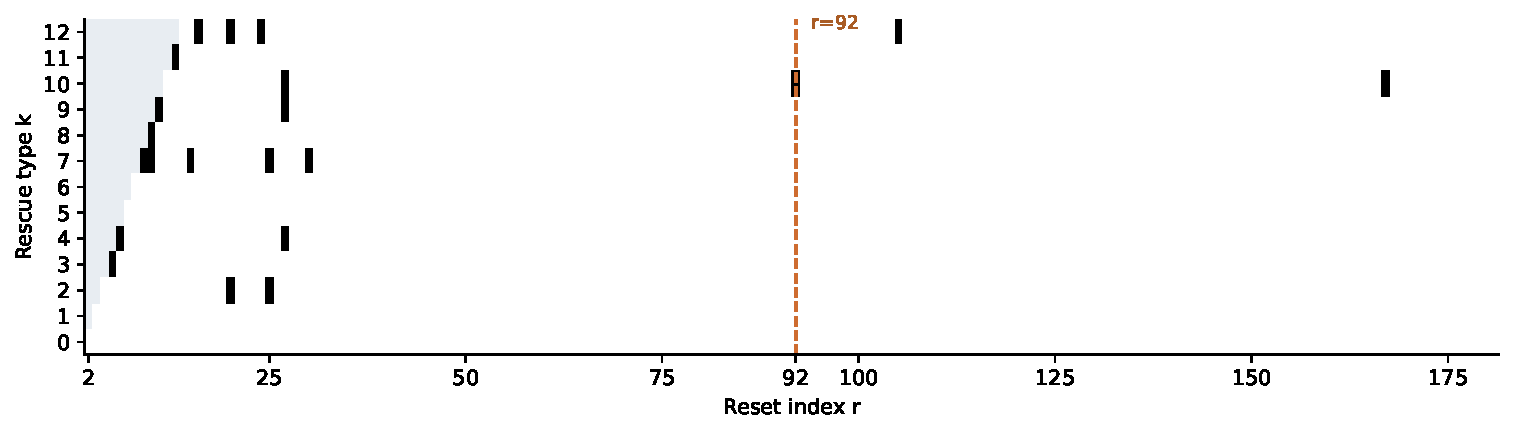
\includegraphics[width=.92\linewidth]{figures/type_zero_heatmap.pdf}
\caption{Zeros (dark squares) for the first thirteen types over the first 180 admissible indices, computed from the archived type-count array. The vertical marker indicates $r=92$.}
\label{fig:heat}
\end{figure}

\section{What a type induction would need to prove}
Define the aggregate rescue count through type $K$ by
\begin{equation}
 \mathcal R_K(r)=\sum_{k=0}^K R_k(r).
\end{equation}
From Proposition~\ref{prop:sufficient}, $\mathcal R_K(r)>0$ is sufficient for replenishment at the complete reset immediately before $6r+4$.

\begin{conjecture}[Bounded-type renewal]\label{conj:renewal}
There are absolute constants $K_0$ and $r_0$ such that
\begin{equation}\label{eq:renewal}
 \boxed{\displaystyle \mathcal R_{K_0}(r)>0\quad\text{for all }r\ge r_0.}
\end{equation}
\end{conjecture}
The case $K_0=0$ is the lower-twin/lower-cousin convolution conjecture. For arbitrary fixed $K_0$, \eqref{eq:renewal} remains a strong prime-quadruple covering conjecture; it does not follow from Theorem~\ref{thm:uniform}.

A putative inductive proof might use a state vector
\begin{equation}
 \mathbf R(r)=(R_0(r),R_1(r),\ldots,R_{K_0}(r))^{\mathsf T}
\end{equation}
and seek a renewal implication between $\mathbf R(r)$ and $\mathbf R(r+1)$. There are two genuine algebraic restrictions:
\begin{enumerate}[label=(\roman*),leftmargin=26pt]
 \item individual prime tiles force all four of their associated sums, including the two consecutive central targets;
 \item different types share some prime forms or encounter incompatible modular restrictions, as in Proposition~\ref{prop:mod5}.
\end{enumerate}
Neither restriction yields a lower bound for $\mathcal R_{K_0}(r+1)$ from $\mathcal R_{K_0}(r)$ alone.  The sum identity \eqref{eq:conservation} is also not a renewal law: it explicitly involves the target population one is trying to prove nonempty.

For a precise sieve formulation, choose a finite-sieve threshold $y$ and write
\begin{equation}
 \mathcal R_K^{\mathrm{cent}}(r)
 =\sum_{k=0}^K W_{k,y}(r)-\mathcal D_{K,y}(r),
\end{equation}
where $\mathcal D_{K,y}(r)$ counts, \emph{with type and starting index multiplicity}, the small-prime survivors for which at least one of the four forms is composite.  Therefore a sufficient condition is
\begin{equation}\label{eq:missing}
 \boxed{\displaystyle
 \mathcal D_{K,y}(r)<\sum_{k=0}^K W_{k,y}(r).}
\end{equation}
Theorem~\ref{thm:uniform} bounds the right-hand side for $k\le\theta r$; no matching uniform upper bound for the left-hand side is known.  In particular, local mutual exclusion of two types does not establish that either type contains a prime quadruple.

\section{Conclusion}
The type formalism adds information absent from the mere indicator of Goldbach representability: it distinguishes endpoint-preserving transitions, two-endpoint replacements, and different gap channels. The resulting convolution and imbalance identities are exact; every type is locally admissible, and linearly many types simultaneously possess abundant small-prime sieve survivors.  Cross-type congruence obstructions produce a nontrivial correlation geometry, while the computations show considerable empirical redundancy.

The mathematical bottleneck is clear.  The arithmetic of the actual primes must force \emph{new} type populations to appear, rather than merely transport already existing four-prime tiles.  Establishing a multitype renewal inequality such as \eqref{eq:missing} or Conjecture~\ref{conj:renewal} would represent a major advance; it cannot be inferred from the current local and algebraic results.  We regard the framework as a source of testable conjectures and exact identities, not as a proof of Goldbach.

\section*{Computational reproducibility}
The source package includes the original FFT-based thirteen-type scanner, its compressed count array, and an independent direct-primality verifier for the $r=92$ example and the local singular-series corrections.  Table~\ref{tab:zeros} and Figure~\ref{fig:heat} can be reproduced from these materials.  No inference about indices beyond the tested range is made.

\bibliographystyle{plainnat}
\bibliography{references}
\end{document}
